\chapter{NEOS}
This chapter compares the \ac{neos} approach to established methods by evaluating expected upper cross-section limits on the boosted \ac{vbf} $HH\rightarrow4b$ analysis. This evaluation employs \ac{neos} in what this thesis terms `autoanalysis', wherein only the most basic selections of reconstructed objects that encapsulate the process of interest are used, while \ac{neos} optimizes cuts considered useful when simultaneously finding the model with the best limits with given uncertainties. This evaluation refrains from unblinding observed collision data as the dominant uncertainties are conservatively estimated and not calibrated at the time of writing. This chapter aims to provide a fair comparison, present the potential \ac{neos} offers compared to more traditional methods and validate it as a robust method.

Cross-section upper limits are obtained with a maximum likelihood fit as explained in chapter \ref{sec:statistics}. \ac{neos} is compared against limits from using the Higgs pair invariant mass $m_{HH}$ and a classifier \ac{nn} trained on separation for signal to background with a \ac{bce} loss function as of equation \ref{eq:bce}. Models are trained with the \ac{tomatos} \ac{nn} training framework developed for this purpose \citep{tomatos} described in section \ref{sec:neos_training}. Both the training for \ac{neos} as well as the classifier use the same \ac{nn} architecture described in \ref{sec:event_classification}, and the hyperparameters are kept consistent to ensure a fair comparison.

Each fit only uses uncertainties which display at least in one bin a 0.5\% difference to the nominal histogram. The reduced set used for optimizing \ac{neos} is summarized in table \ref{tab:neos-samples}, chosen from the highest-ranked uncertainties of an $m_{HH}$ fit that incorporated the full set of uncertainties. Figure \ref{fig:m_hh_neos_unc_ranking} shows a ranking of these uncertainties. The complete ranked list of uncertainties for the \mhh fit is available in Appendix \ref{fig:m_hh_full_sys_ranking}. The \ac{pdf}+$\alpha_s$ uncertainty, however, was excluded from the \ac{neos} optimization due to its minimal impact relative to the computational overhead of processing 100 additional samples. $t\overline{t}$ as a background is neglected entirely as it contributes 1-2\% to the event selection and has no effect when determining cross-section limits.

\begin{figure}
    \centering
    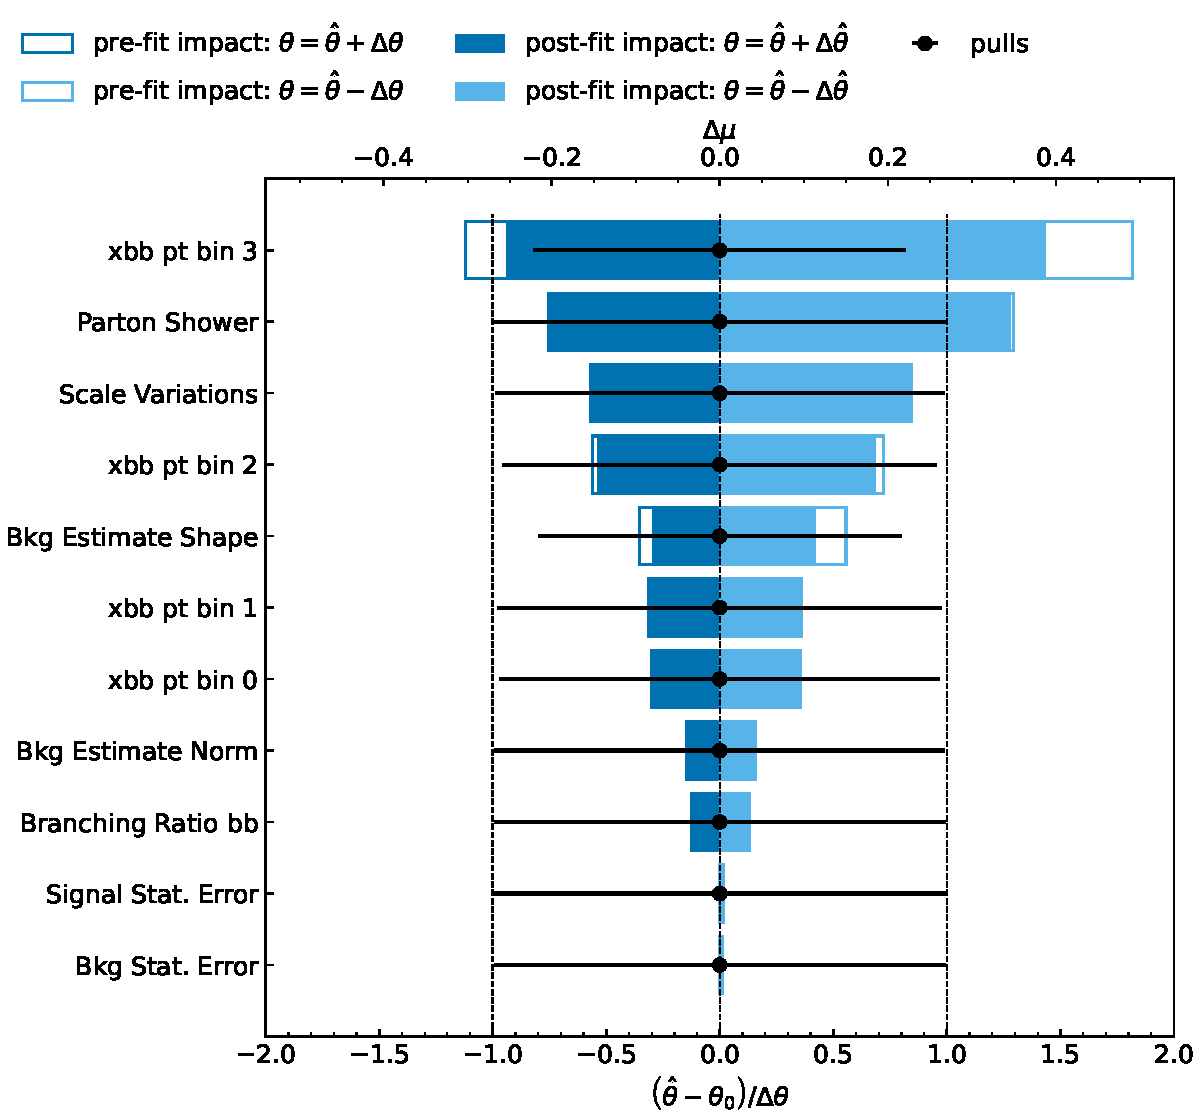
\includegraphics[width=0.95\textwidth]{neos_results/m_hh_neos_unc_ranking.pdf}
    \caption[]{Ranking of selected uncertainties used in the training for \ac{neos} ordered by their post-fit impact on the signal strength, $\Delta\mu$, displayed on the upper axis for an invariant Higgs Pair mass maximum likelihood fit (\mhh{}). The impact of a nuisance parameter $\Theta$ is assessed by performing four fits. In each fit, the parameter $\Theta$ is fixed to its nominal best-fit value $\hat{\Theta}$ plus a given nuisance parameter uncertainty $\Delta\Theta$. The difference between the resulting fitted signal strength $\mu_\text{fit}$ and the nominal best-fitted value is then computed as $\Delta\mu=\hat{\mu} - \mu_\text{fit}$. This process is repeated for pre-fit $\pm\Delta\Theta$ and post-fit $\pm\Delta\hat{\Theta}$ uncertainties of $\Theta$. The lower axis and the black points represent the pull for each nuisance paramter, calculated as the difference between the best-fit value and the nominal pre-fit $(\hat{\Theta} - \Theta_0)$, divided by its variance $\Delta\Theta$ for the parameter $\Theta$. If the model is accurate, the expected value of each pull should be zero, with a variance of one, in the asymptotic limit. In this limit the test statistic is computed from the sum of pulls and follows a $\chi^2$ distribution if the model is correct. Therefore, pulls serve as goodness-of-fit quantities. }
    \label{fig:m_hh_neos_unc_ranking}
\end{figure}




\section{Training Evaluation}
Figure \ref{fig:training_metrics_validation} presents the training loss and Asimov significance per epoch and as well histograms of the final model evaluated on the samples from table \ref{tab:neos-samples} for both the \ac{bce}-trained \ac{nn} and the neos \ac{nn}. The \ac{bce}-trained model converges for the validation dataset at about epoch 500, while the \ac{neos} model converges at about epoch 1500. The best validated epoch for the \ac{bce}-trained \ac{nn} is 993, and for the \ac{neos}-trained \ac{nn} it is 1986.

The \ac{bce}-trained \ac{nn} exhibits typical classifier behavior, with most background events in the lowest bin and decreasing event counts in higher binsWhen evaluated on signal samples, the behavior is reversed, with the largest impact of uncertainties on the signal occurring in the last bin.

In contrast, the \ac{neos}-trained \ac{nn} exhibits a different behavior. The typical interpretation of the \ac{nn} score, where small values correspond to background and large values correspond to signal, becomes less straightforward. When uncertainties are taken into account, the score distribution adopts a non-trivial shape, spreading the signal across all bins in an alternating pattern. Despite this, there remains a general trend of separating background and signal, although not in the conventional manner.

The optimization still seeks to isolate signal from background particularly evident in the first and third bins, which contain almost no background events, thereby benefiting the statistical test. For this training, the smallest bandwidth for the kernel density estimate \ac{kde} that maintains a learning gradient is 0.2. Figure \ref{fig:neos_valid_kde_hists} demonstrates that the binned kernel density estimates are a rough approximation compared to the evaluated model shown in figure \ref{fig:neos_hist}, underscoring this parameters critical role in this optimization.

Moreover, the Asimov significance, as defined in equation \ref{eq:asimov-significance} and commonly used as a proxy for statistical testing during analysis optimization, is correlated with the optimization for both training methods. The \ac{neos} training displays a $\sim\qty[]{30}{\percent}$ larger significance compared to the \ac{bce} training.

\begin{figure}
    \centering
    \subfigure[]{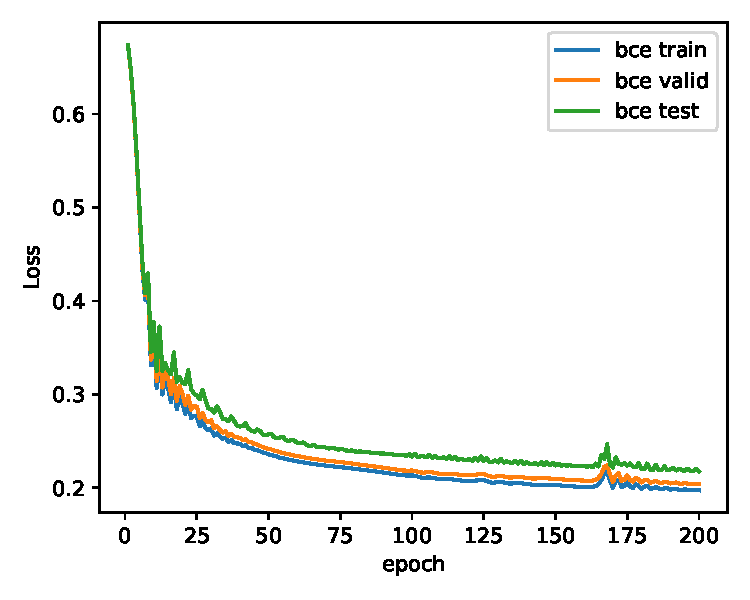
\includegraphics[width=.45\textwidth]{neos_results/tomatos_bce_5_1000/bce.pdf}}
    \subfigure[]{\includegraphics[width=.45\textwidth]{neos_results/tomatos_cls_5_2500_slope_50/cls.pdf}} \label{fig:neos_validation_loss}\\
    \subfigure[]{\includegraphics[width=.45\textwidth]{neos_results/tomatos_bce_5_1000/hist.pdf}}
    \subfigure[]{\includegraphics[width=.45\textwidth]{neos_results/tomatos_cls_5_2500_slope_50/hist.pdf}} \label{fig:neos_hist}\\
    \subfigure[]{\includegraphics[width=.45\textwidth]{neos_results/tomatos_bce_5_1000/Z_A.pdf}}
    \subfigure[]{\includegraphics[width=.45\textwidth]{neos_results/tomatos_cls_5_2500_slope_50/Z_A.pdf}} \\
    \caption[]{\textbf{(Left Column)} \ac{nn} trained with a \ac{bce} loss function. \textbf{(Right Coloumn)} \ac{nn} trained with \ac{neos}.  \textbf{(Top To bottom)}: Loss function evaluated on training, validation and test dataset per training epoch, histogrammed \ac{nn} score for samples used in the training (nominal signal (\hexline{ff7f0e}), background estimate (\hexline{1f77b4})) and Asimov significance. Displayed uncertainties are all signal related.}
    \label{fig:training_metrics_validation}
\end{figure}


\begin{figure}
    \centering
    \subfigure[]{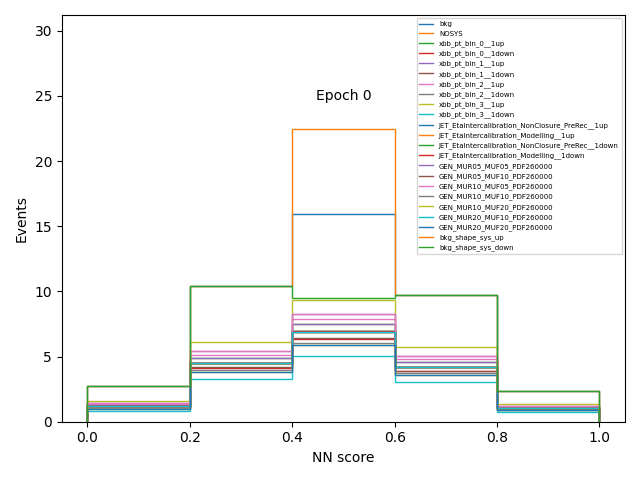
\includegraphics[width=.47\textwidth]{neos_results/tomatos_cls_5_2500_slope_50/0000.png}}
    \subfigure[]{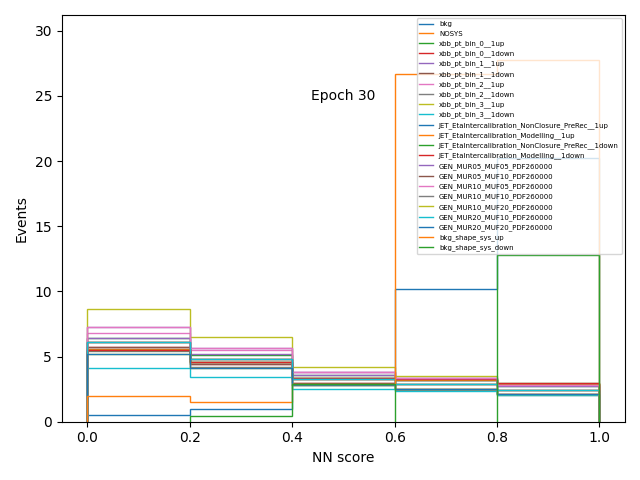
\includegraphics[width=.47\textwidth]{neos_results/tomatos_cls_5_2500_slope_50/0030.png}}\\
    \subfigure[]{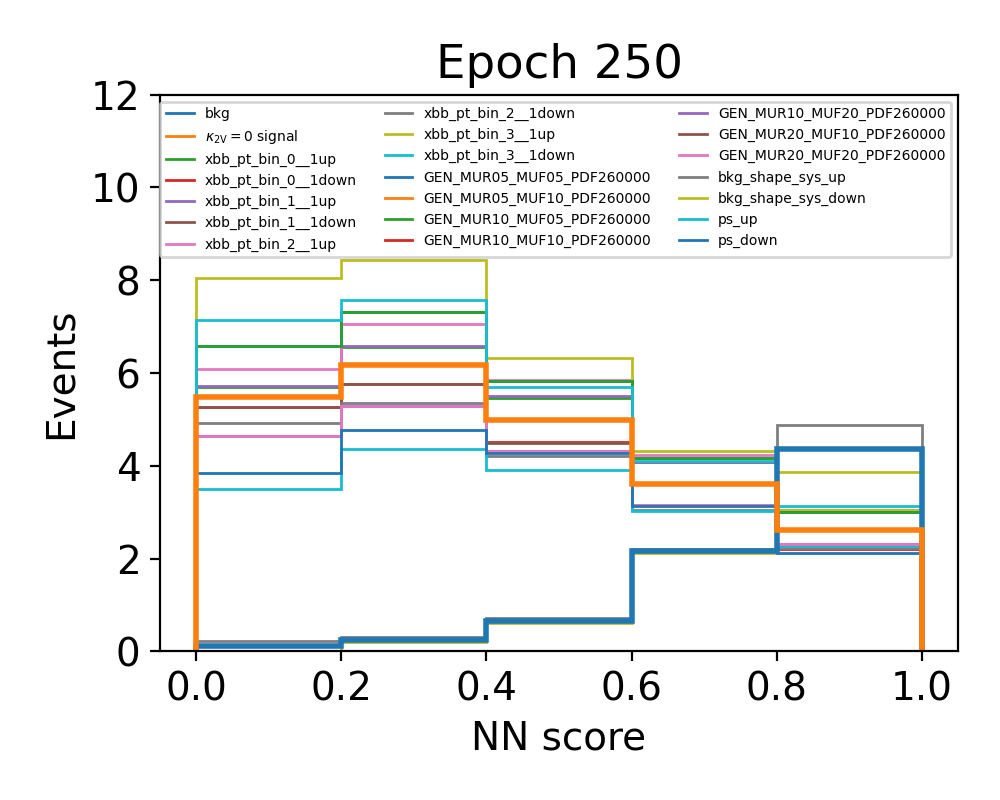
\includegraphics[width=.47\textwidth]{neos_results/tomatos_cls_5_2500_slope_50/0250.png}}
    \subfigure[]{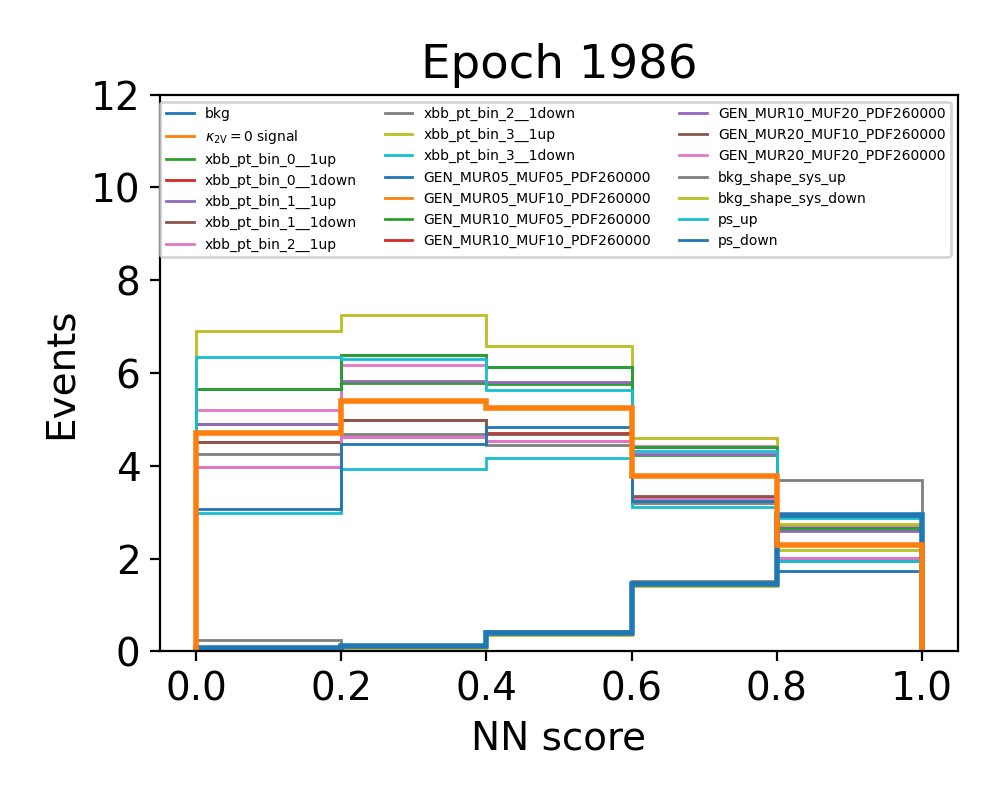
\includegraphics[width=.47\textwidth]{neos_results/tomatos_cls_5_2500_slope_50/1986.png}}
    \caption[]{Binned kernel density estimates used by \ac{neos} evaluated at different training epochs for a bandwidth of 0.2.}
    \label{fig:neos_valid_kde_hists}
\end{figure}



\subsection{Uncertainty Optimization}

The uncertainty ranking presented in figure \ref{fig:m_hh_neos_unc_ranking} highlights that the GN2X version of the $X \rightarrow bb$ tagger uncertainties, along with parton shower and scale variation uncertainties, are the primary uncertainties affecting the signal. For the background estimate, the dominant uncertainties are the shape and normalization uncertainties. A detailed description to these uncertainties are found in \ref{ch:systematics}.


The shape of the \ac{neos} histogram becomes intuitive when observing the uncertainties during training. Events with large uncertainties on the signal predominantly appear in the first bin, which seem less useful for discovery. The second to fourth bins demonstrate the most discovery potential, with substantial signals compared to the background, while most background events are distributed in the last bin.

Figure \ref{fig:neos_unc_dev} illustrates the evolution of representative uncertainties derived from binned kernel density estimates, as the ones shown in figure \ref{fig:neos_valid_kde_hists}  used during \ac{neos}' training. The most dominant uncertainty is the third \pt bin of the GN2X version of the $X \rightarrow bb$ tagger which has a strong tendency to be placed in lower bins most dominantly in the first bin. This is due to its clear signature, characterized by high kinetic energy and large GN2X tagger scores.


The minimization and redistribution capability are more pronounced with uncertainties affecting most events, such as the alternative parton shower uncertainty on the signal or the shape uncertainty on the background extracted from the histogram shape in the \ac{vr}, accessible to \ac{neos} during training. The development of the parton shower uncertainty, shown in figure \ref{fig:neos_unc_dev_ps}, indicates a reduction of the signal uncertainty in the second to fourth bins, which have the highest signal-to-background ratio, while uncertainties increase in the first and last bins.


The development of the background shape uncertainty further emphasizes this behavior. Here, bins three, four, and five are the relevant ones for the background estimate. Bins three and four, with the strongest power for discovery, decrease the error on the kernel density estimates almost to zero, while bin five remains about constant, and bins one and two experience significant increases. These observations suggest that the first bin may act as a container for events with large uncertainties.




\begin{figure}
    \centering
    \subfigure[]{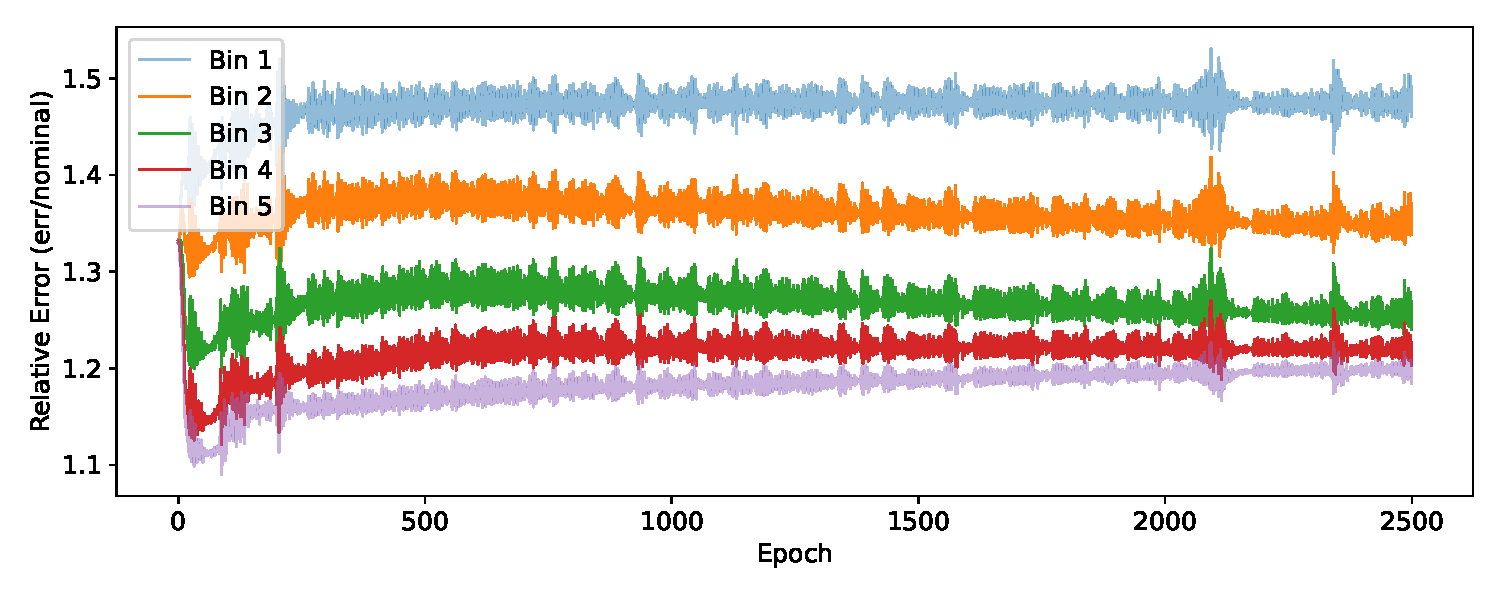
\includegraphics[width=.94\textwidth]{neos_results/tomatos_cls_5_2500_slope_50/xbb_pt_bin_3_rel_error.pdf}}\\
    \subfigure[]{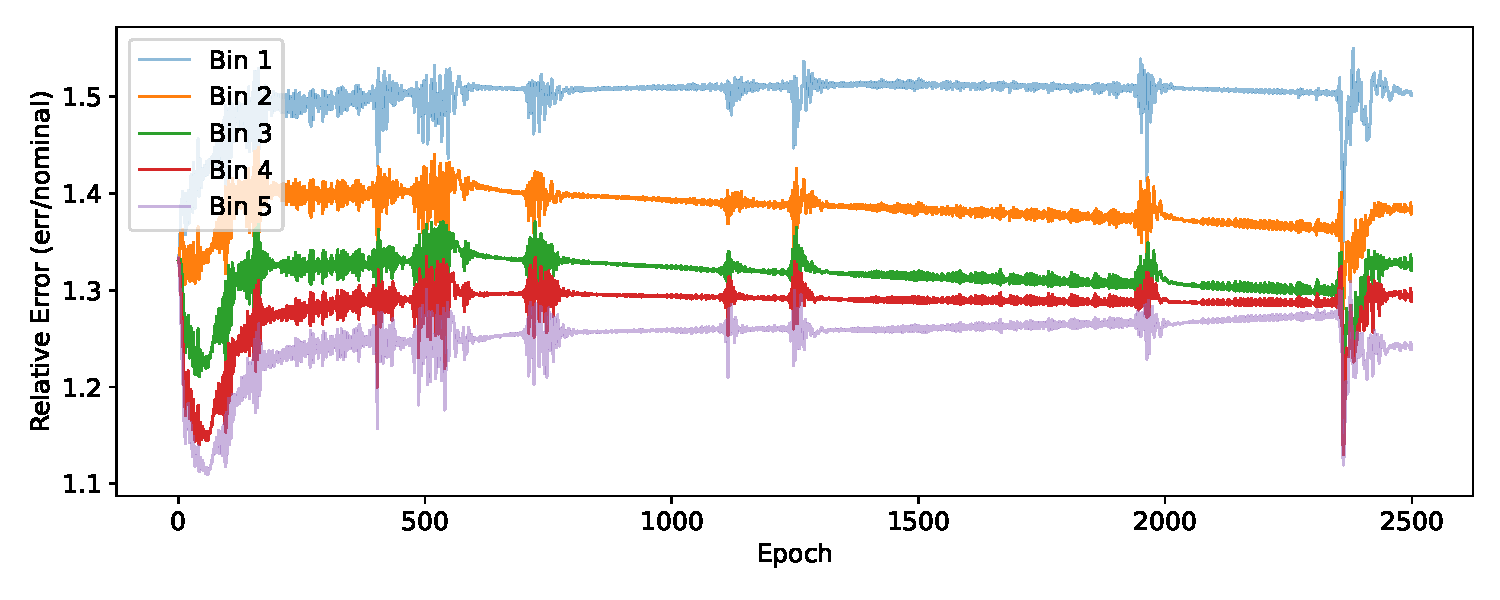
\includegraphics[width=.94\textwidth]{neos_results/tomatos_cls_5_2500_slope_50/ps_rel_error.pdf}}\\     \label{fig:neos_unc_dev_ps}
    \subfigure[]{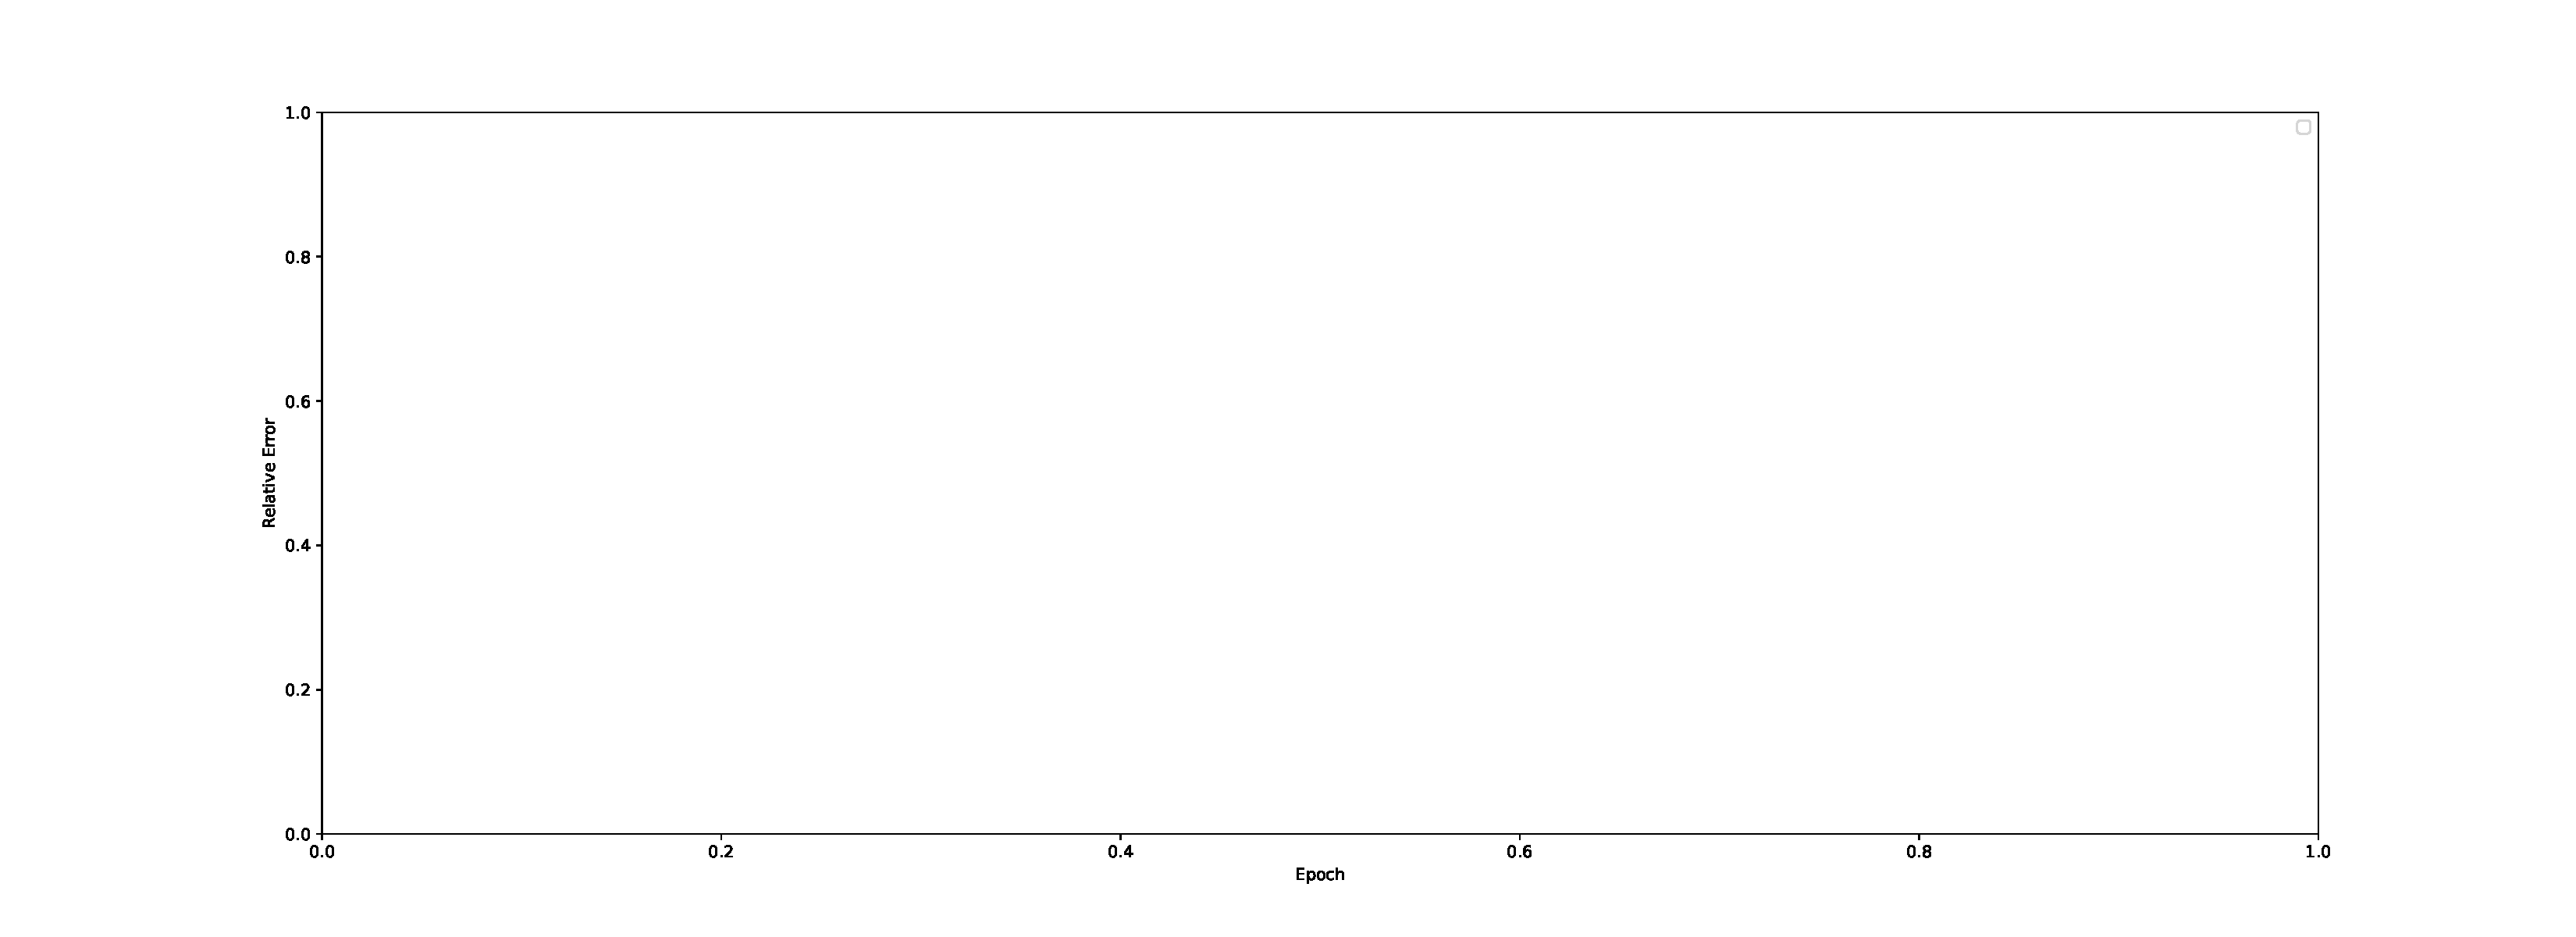
\includegraphics[width=.94\textwidth]{neos_results/tomatos_cls_5_2500_slope_50/bkg_shape_sys_rel_error.pdf}}     \label{fig:neos_unc_dev_bkg_shape_sys}
    \caption[]{Relative error per bin for the: (a) third \pt bin GN2X version of the $X\rightarrow bb$ tagger (b) background shape uncertainty to the nominal background estimate and (c) alternative parton shower uncertainty on the signal.}
    \label{fig:neos_unc_dev}
\end{figure}

\subsection{Cuts Optimization}
To determine the $m_{jj}$ and $|\Delta\eta(j,j)|$ cuts on the \ac{vbf} jets  for the \mhh and \ac{bce}-trained \ac{nn} a scan of cut values was performed. For each cut value, the Asimov significance of the resulting histogram was calculated. Figure \ref{fig:cut_scan} presents the results of this procedure depending on the cuts while table \ref{tab:z_a_cuts} displays the derived cuts from maximizing the Asimov significance. For comparison, cuts optimized using the Asimov significance for the \ac{neos} model are also included.

Cuts found by the \ac{neos} optimization as explained in \ref{sec:neos_training} are shown in figure \ref{fig:neos_cuts} and converge at about epoch 1000. The stability of the training process is critically dependent on the chosen slope $m$ of the sigmoid function $1/(1+e^{-mx})$  used to approximatively model the cut in a differentiable manner, as illustrated in figures \ref{fig:slope_study_1} and \ref{fig:slope_study_2}. A larger slope provides a better approximation but results in a steeper gradient. If the slope is too large, here $\gtrsim 100$, the training becomes unstable as the optimizer struggles to find the gradient. This is also because even though it is just two optimization parameters each of the eight to be processed sample adds a sigmoid to the automatic differentiation. The smoothest training with a slope of 50 is chosen which optimizes both cuts and displays a smooth loss function for the evaluation samples.

However it is not necessarily disadvantageous if one of the cuts is deactivated in favor of the other, as they are correlated. Figure \ref{fig:vbf_correlation} shows this correlation, with a Pearson correlation coefficient of $\rho_{m_{jj},|\Delta\eta(j,j)|}=0.73$. Additionally, scanning the cuts in the direction of reducing data is beneficial for the training as it is presented with all training examples from the beginning.

It is noted that the choice of a slope of 50 introduces significant variability in the actual cut value, as shown in figure \ref{fig:sigmoid_slope_50}. The min-max scaling places the parameter range between 0 and 1. The $\Delta x$ of the cut, representing the central value of the sigmoid and when the sigmoid reaches 95\% selection efficiency, is $\Delta x=0.059$. When unscaled to the $m_{jj}$ range, and considering twice the $\Delta x$ range to cover 0.05 and 0.95 cutting efficiency, it results in $\Delta m_{jj}\approx \qty[]{900}{GeV}$. This might lead to an underestimation of the true optimal cut value.

\begin{figure}
    \centering
    \subfigure[]{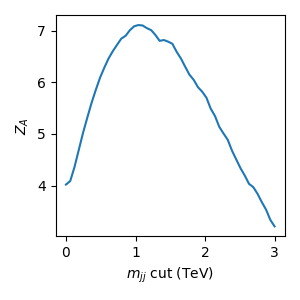
\includegraphics[width=.3\textwidth]{neos_results/s_b_optimization/s_b_optimization_m_hh_5_m_jj}}
    \subfigure[]{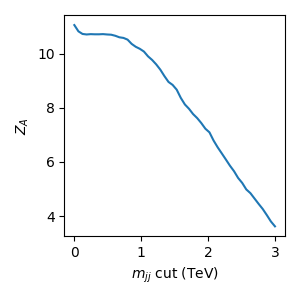
\includegraphics[width=.3\textwidth]{neos_results/s_b_optimization/s_b_optimization_tomatos_bce_5_1000_m_jj}}
    \subfigure[]{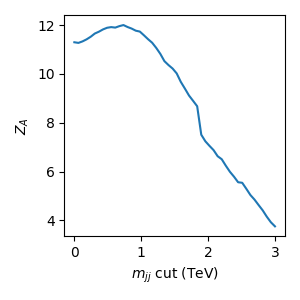
\includegraphics[width=.3\textwidth]{neos_results/s_b_optimization/s_b_optimization_tomatos_cls_5_2500_slope_50_m_jj}}\\
    \subfigure[]{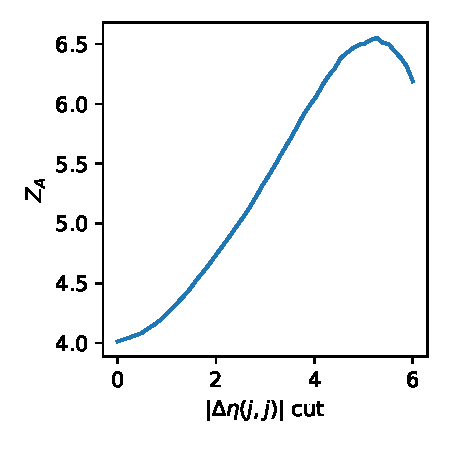
\includegraphics[width=.3\textwidth]{neos_results/s_b_optimization/s_b_optimization_m_hh_5_eta_jj}}
    \subfigure[]{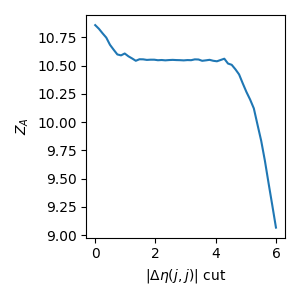
\includegraphics[width=.3\textwidth]{neos_results/s_b_optimization/s_b_optimization_tomatos_bce_5_1000_eta_jj}}
    \subfigure[]{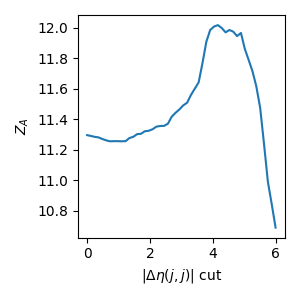
\includegraphics[width=.3\textwidth]{neos_results/s_b_optimization/s_b_optimization_tomatos_cls_5_2500_slope_50_eta_jj}}
    \caption[]{Columns left to right: $\mhh$, \ac{bce}-trained \ac{nn}, \ac{neos}-trained \ac{nn}: Asimov Significances after applying a cut on \textbf{(a)-(c)} on the invariant mass $m_{jj}$ and \textbf{(d)-(f)} the pseudorapidity separation $|\Delta\eta(j,j)|$ of the \ac{vbf} jets. }
    \label{fig:cut_scan}
\end{figure}

\begin{figure}
    \centering
    \includegraphics[width=.6\textwidth]{neos_results/tomatos_cls_5_2500_slope_50/cuts}
    \caption[]{Optimized \ac{neos} cuts per epoch for the invariant mass $m_{jj}$ and the pseudorapidity difference $|\Delta\eta(j,j)|$ of the two \ac{vbf} jets.}
    \label{fig:neos_cuts}
\end{figure}

\begin{table}[]\label{tab:z_a_cuts}
    \centering
    \caption{Optimized cuts for \mhh and the trained \acp{nn} from the maximized Asimov significances shown in figure \ref{fig:cut_scan} and the cuts found by the \ac{neos} optimization in epoch 185 of figure \ref{fig:neos_cuts}.}
    \begin{tabular}{c|c|c}
                                  & $m_{jj}$ (GeV) & $|\Delta\eta(j,j)|$ \\\hline
        \mhh                      & >1041          & >5.27               \\
        \ac{bce}-trained \ac{nn}  & >0             & >0                  \\
        \ac{neos}-trained \ac{nn} & >735           & >4.16               \\ \hline
        found by \ac{neos}        & >618           & >4.3                \\
    \end{tabular}
\end{table}



\begin{figure}
    % \captionsetup[subfigure]{labelformat=empty, skip=0pt}
    \centering
    \subfigure[]{\includegraphics[width=.33\textwidth]{neos_results/tomatos_cls_5_200_slope_25/cls.pdf}}
    \subfigure[]{\includegraphics[width=.33\textwidth]{neos_results/tomatos_cls_5_200_slope_25/cuts.pdf}}\\
    \subfigure[]{\includegraphics[width=.33\textwidth]{neos_results/tomatos_cls_5_200_slope_50/cls.pdf}}
    \subfigure[]{\includegraphics[width=.33\textwidth]{neos_results/tomatos_cls_5_200_slope_50/cuts.pdf}}\\
    \subfigure[]{\includegraphics[width=.33\textwidth]{neos_results/tomatos_cls_5_200_slope_75/cls.pdf}}
    \subfigure[]{\includegraphics[width=.33\textwidth]{neos_results/tomatos_cls_5_200_slope_75/cuts.pdf}}\\
    \subfigure[]{\includegraphics[width=.33\textwidth]{neos_results/tomatos_cls_5_200_slope_100/cls.pdf}}
    \subfigure[]{\includegraphics[width=.33\textwidth]{neos_results/tomatos_cls_5_200_slope_100/cuts.pdf}}\\
    \caption[]{(1/2) Loss functions on the left and optimized cuts on the right hand side per \ac{neos} training epoch with a sigmoid slope of 25, 50, 75, 100.}
    \label{fig:slope_study_1}
\end{figure}

\begin{figure}
    \centering
    \subfigure[]{\includegraphics[width=.33\textwidth]{neos_results/tomatos_cls_5_200_slope_500/cls.pdf}}
    \subfigure[]{\includegraphics[width=.33\textwidth]{neos_results/tomatos_cls_5_200_slope_500/cuts.pdf}}\\
    \subfigure[]{\includegraphics[width=.33\textwidth]{neos_results/tomatos_cls_5_200_slope_1000/cls.pdf}}
    \subfigure[]{\includegraphics[width=.33\textwidth]{neos_results/tomatos_cls_5_200_slope_1000/cuts.pdf}}\\
    \subfigure[]{\includegraphics[width=.33\textwidth]{neos_results/tomatos_cls_5_200_slope_5000/cls.pdf}}
    \subfigure[]{\includegraphics[width=.33\textwidth]{neos_results/tomatos_cls_5_200_slope_5000/cuts.pdf}}\\
    \subfigure[]{\includegraphics[width=.33\textwidth]{neos_results/tomatos_cls_5_200_slope_10000/cls.pdf}}
    \subfigure[]{\includegraphics[width=.33\textwidth]{neos_results/tomatos_cls_5_200_slope_10000/cuts.pdf}}\\
    \caption[]{(2/2) Loss functions on the left and optimized cuts on the right hand side per \ac{neos} training epoch with a sigmoid slope of 500, 1000, 5000, 10000.}
    \label{fig:slope_study_2}
\end{figure}


% \begin{figure}
%     \centering
%     \subfigure[]{\includegraphics[width=.3\textwidth]{neos_results/tomatos_cls_5_1000_slope_50/cls.pdf}}
%     \subfigure[]{\includegraphics[width=.3\textwidth]{neos_results/tomatos_cls_5_1000_slope_500/cls.pdf}}
%     \subfigure[]{\includegraphics[width=.3\textwidth]{neos_results/tomatos_cls_5_1000_slope_1000/cls.pdf}} \\
%     \caption[]{Loss functions from left to right for \ac{neos} training with a sigmoid slope of 50, 500, 1000.}
%     \label{fig:slope_study}
% \end{figure}


\begin{figure}
    \centering
    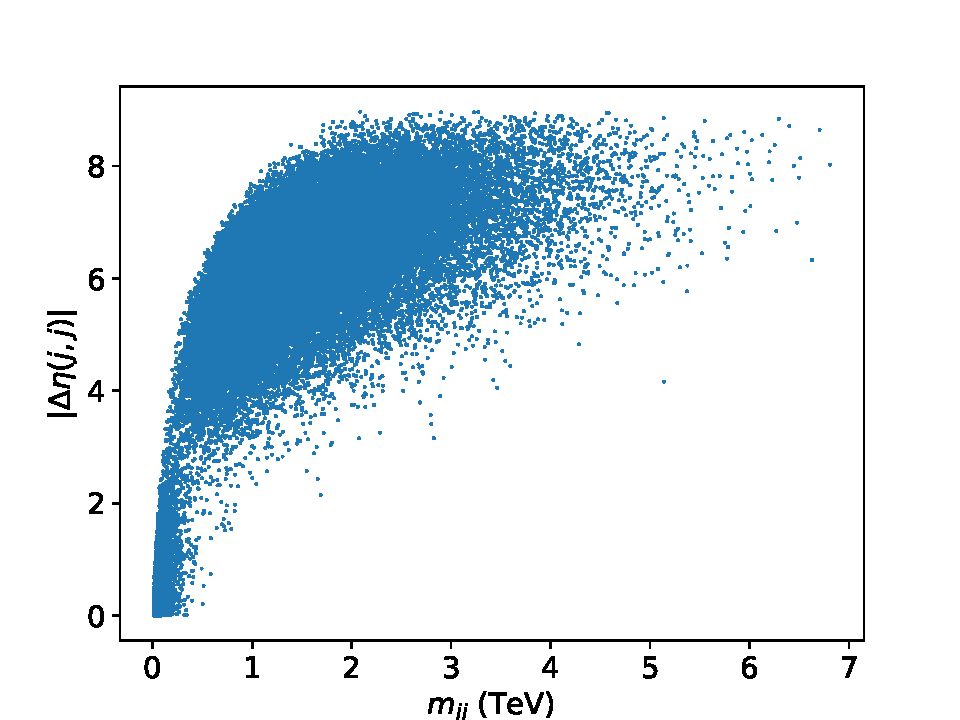
\includegraphics[width=.5\textwidth]{neos_results/vbf_correlation.pdf}
    \caption[]{Correlation between the invariant mass of the \ac{vbf} jet system $m_{jj}$ and their pseudorapidity difference $|\Delta\eta(j,j)|$.}
    \label{fig:vbf_correlation}
\end{figure}

\begin{figure}
    \centering
    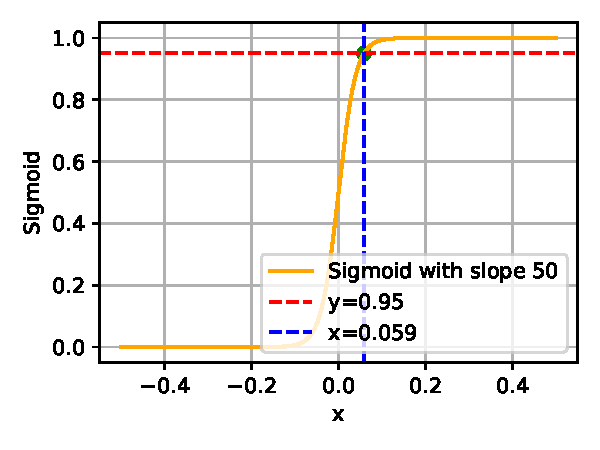
\includegraphics[width=.5\textwidth]{sigmoid_slope_50.pdf}
    \caption[]{Sigmoid used as approximation of the cuts with a slope of 50. Lines indicate $x$ and $y$ values for which 95\% selection efficiency is achieved.}
    \label{fig:sigmoid_slope_50}
\end{figure}





\section{Performance Comparison}
After training the \acp{nn} they are evaluated alongside an $\mhh$ fit \textit{without} the use of any \ac{neos} methods to determine limits on the boosted \ac{vbf} $HH\rightarrow4b$ cross-section with the \textit{cabinetry} fitting framework \citep{cranmer_2021_4627038}. Consequently, the event selection, application of cuts, and creation of histograms are performed using traditional methods.

All models use the same methods for the background uncertainty estimation described in \ref{sec:bkg_uncertainties}. Dominating uncertainties are shown in figure \ref{fig:neos_validation_uncertaintes_1} and \ref{fig:neos_validation_uncertaintes_2}. Histograms and their uncertainties are shown in figure \ref{fig:neos_pre_post_fit} before and after fitting. All models display more constrained post-fit uncertainties.

\begin{figure}
    \centering
    \subfigure[]{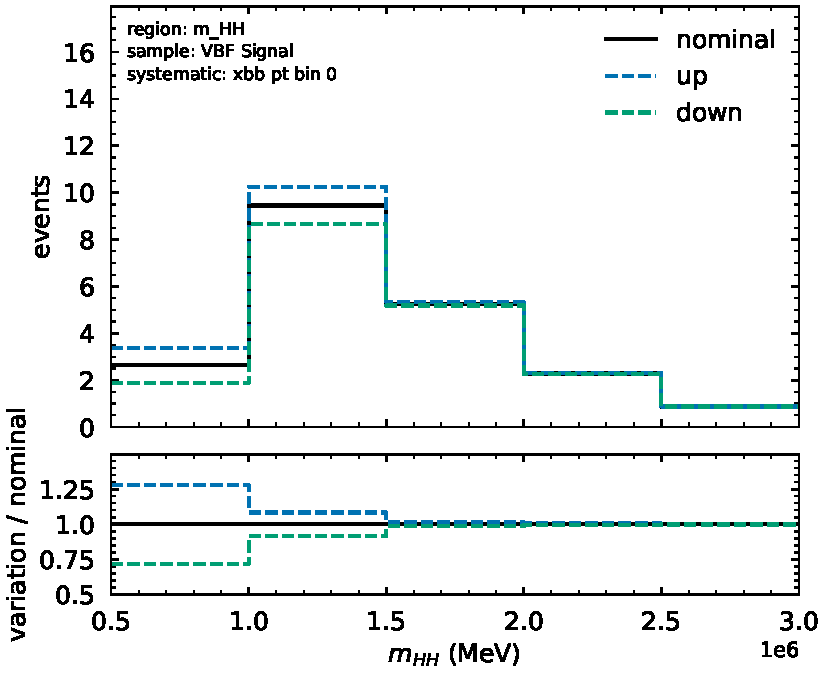
\includegraphics[width=.3\textwidth]{neos_results/m_hh_5_l1cvv0cv1/figures/templates/m_HH_VBF-Signal_xbb-pt-bin-0.pdf}}
    \subfigure[]{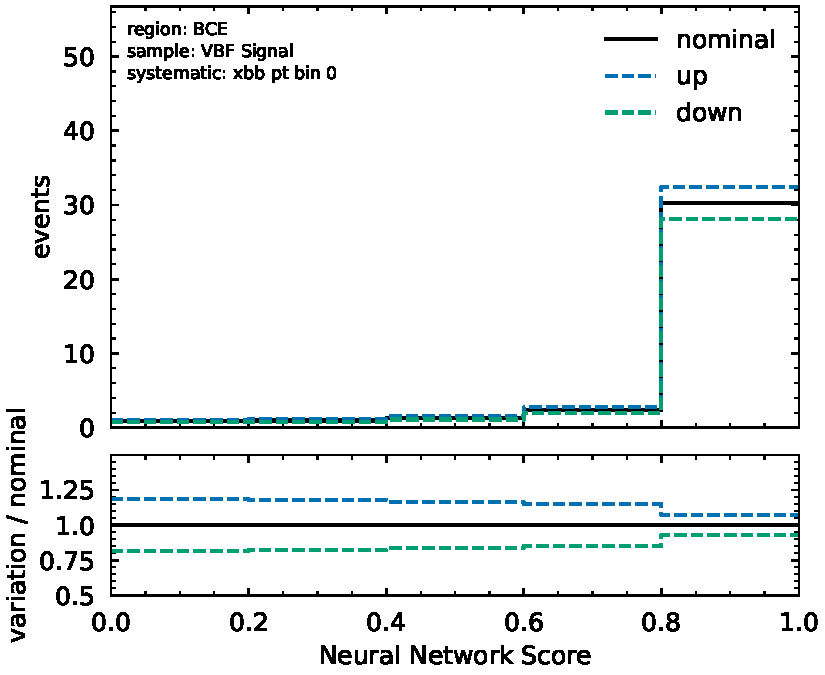
\includegraphics[width=.3\textwidth]{neos_results/tomatos_bce_5_1000_l1cvv0cv1/figures/templates/BCE_VBF-Signal_xbb-pt-bin-0.pdf}}
    \subfigure[]{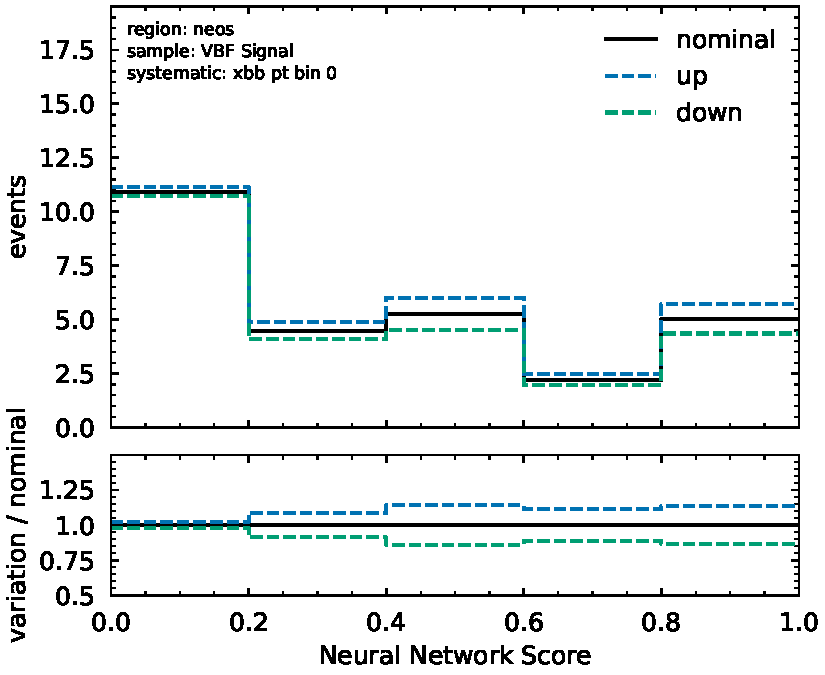
\includegraphics[width=.3\textwidth]{neos_results/tomatos_cls_5_2500_slope_50_l1cvv0cv1/figures/templates/neos_VBF-Signal_xbb-pt-bin-0.pdf}} \\
    \subfigure[]{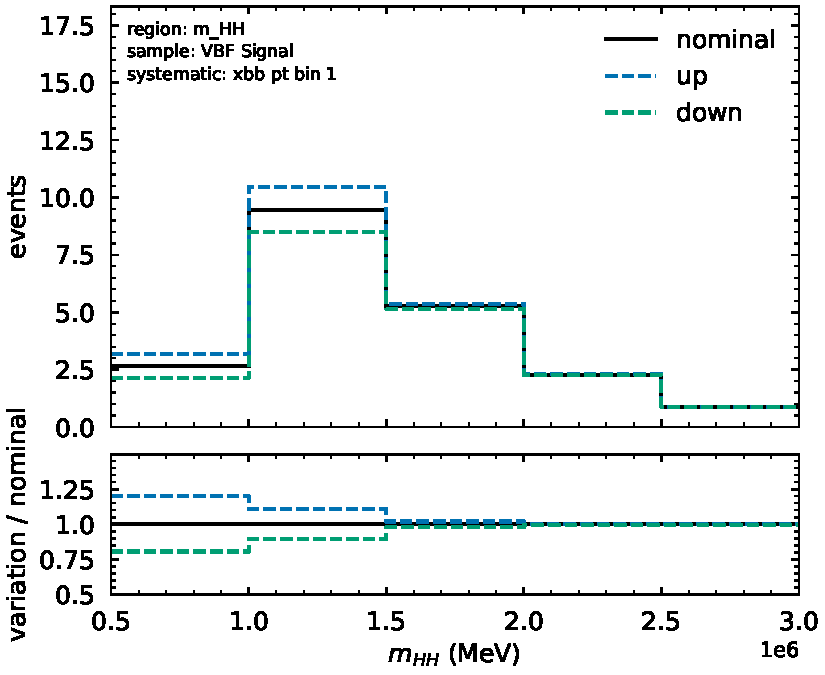
\includegraphics[width=.3\textwidth]{neos_results/m_hh_5_l1cvv0cv1/figures/templates/m_HH_VBF-Signal_xbb-pt-bin-1.pdf}}
    \subfigure[]{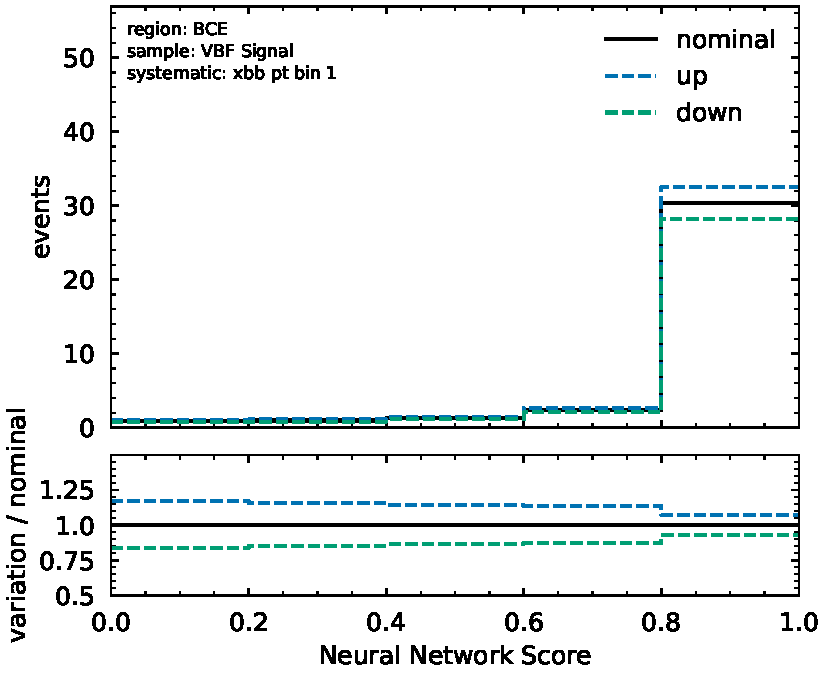
\includegraphics[width=.3\textwidth]{neos_results/tomatos_bce_5_1000_l1cvv0cv1/figures/templates/BCE_VBF-Signal_xbb-pt-bin-1.pdf}}
    \subfigure[]{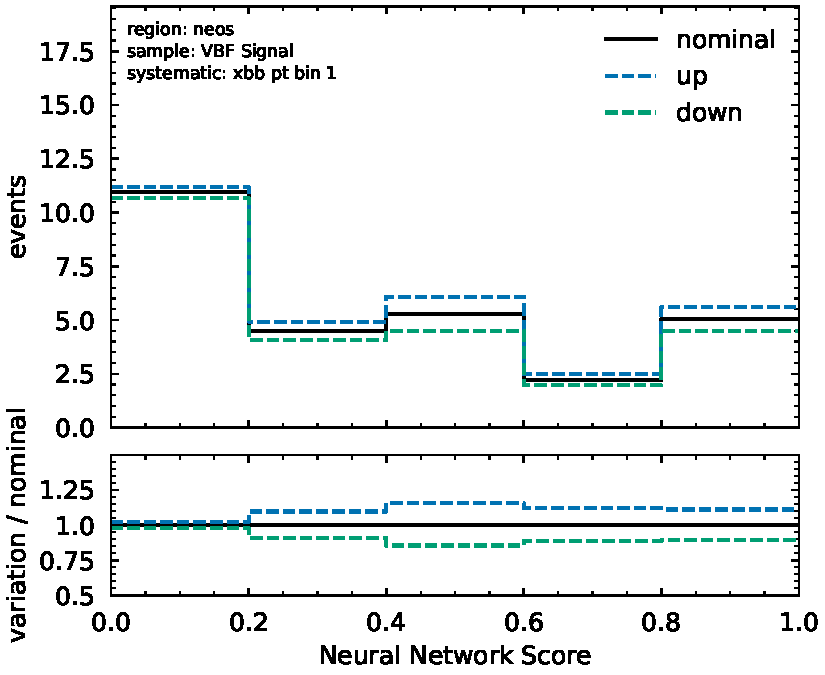
\includegraphics[width=.3\textwidth]{neos_results/tomatos_cls_5_2500_slope_50_l1cvv0cv1/figures/templates/neos_VBF-Signal_xbb-pt-bin-1.pdf}} \\
    \subfigure[]{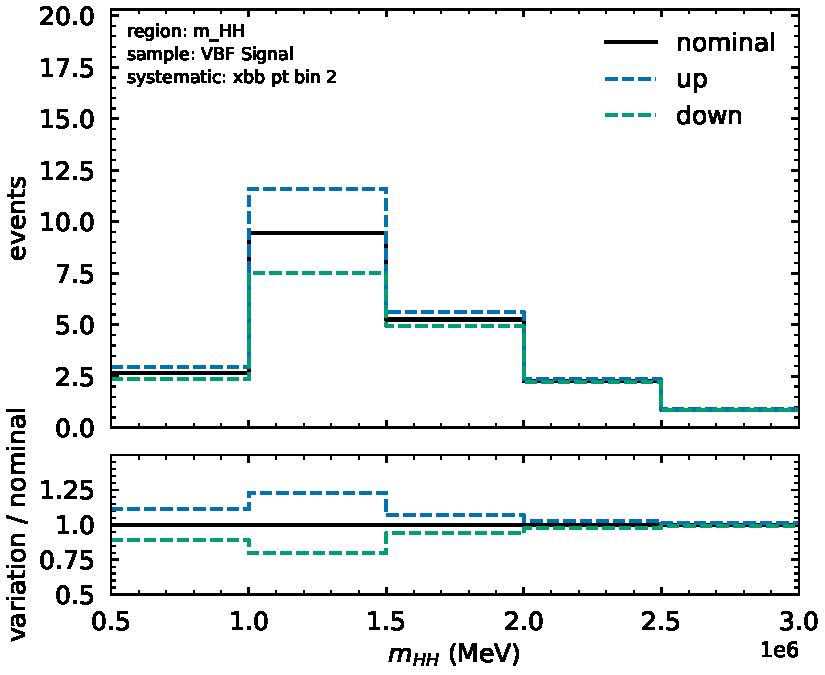
\includegraphics[width=.3\textwidth]{neos_results/m_hh_5_l1cvv0cv1/figures/templates/m_HH_VBF-Signal_xbb-pt-bin-2.pdf}}
    \subfigure[]{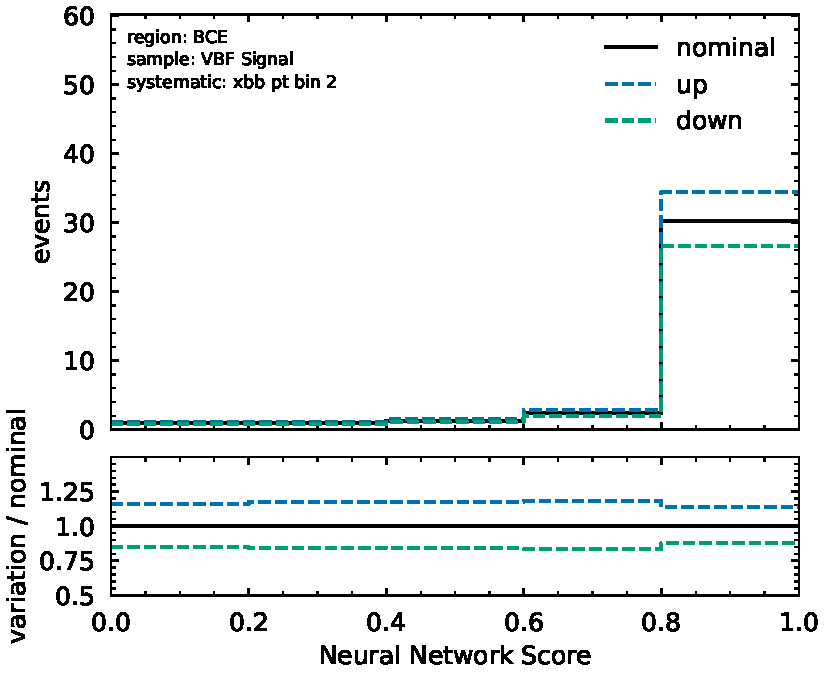
\includegraphics[width=.3\textwidth]{neos_results/tomatos_bce_5_1000_l1cvv0cv1/figures/templates/BCE_VBF-Signal_xbb-pt-bin-2.pdf}}
    \subfigure[]{\includegraphics[width=.3\textwidth]{neos_results/tomatos_cls_5_2500_slope_50_l1cvv0cv1/figures/templates/neos_VBF-Signal_xbb-pt-bin-2.pdf}} \\
    \subfigure[]{\includegraphics[width=.3\textwidth]{neos_results/m_hh_5_l1cvv0cv1/figures/templates/m_HH_VBF-Signal_xbb-pt-bin-3.pdf}}
    \subfigure[]{\includegraphics[width=.3\textwidth]{neos_results/tomatos_bce_5_1000_l1cvv0cv1/figures/templates/BCE_VBF-Signal_xbb-pt-bin-3.pdf}}
    \subfigure[]{\includegraphics[width=.3\textwidth]{neos_results/tomatos_cls_5_2500_slope_50_l1cvv0cv1/figures/templates/neos_VBF-Signal_xbb-pt-bin-3.pdf}} \\
    \caption[]{Uncertainties (1/2) for columns left to right: $\mhh$, \ac{bce}-trained \ac{nn}, \ac{neos}-trained \ac{nn}. Top to bottom: 30\% GN2X scale factor uncertainties for the four bins used in the calibration of the GN2X tagger as shown in figure \ref{fig:xbb_sf}.}
    \label{fig:neos_validation_uncertaintes_1}
\end{figure}
\begin{figure}
    \centering
    \subfigure[]{\includegraphics[width=.3\textwidth]{neos_results/m_hh_5_l1cvv0cv1/figures/templates/m_HH_Background_Bkg-Estimate-Shape.pdf}}
    \subfigure[]{\includegraphics[width=.3\textwidth]{neos_results/tomatos_bce_5_1000_l1cvv0cv1/figures/templates/BCE_Background_Bkg-Estimate-Shape.pdf}}
    \subfigure[]{\includegraphics[width=.3\textwidth]{neos_results/tomatos_cls_5_2500_slope_50_l1cvv0cv1/figures/templates/neos_Background_Bkg-Estimate-Shape.pdf}} \\
    \subfigure[]{\includegraphics[width=.3\textwidth]{neos_results/m_hh_5_l1cvv0cv1/figures/templates/m_HH_VBF-Signal_Scale-Variations.pdf}}
    \subfigure[]{\includegraphics[width=.3\textwidth]{neos_results/tomatos_bce_5_1000_l1cvv0cv1/figures/templates/BCE_VBF-Signal_Scale-Variations}}
    \subfigure[]{\includegraphics[width=.3\textwidth]{neos_results/tomatos_cls_5_2500_slope_50_l1cvv0cv1/figures/templates/neos_VBF-Signal_Scale-Variations.pdf}} \\
    \caption[]{Uncertainties (2/2) for columns left to right: $\mhh$, \ac{bce}-trained \ac{nn}, \ac{neos}-trained \ac{nn}. Top: Background shape uncertainty, Bottom: envelope of scale variations. Details about their estimation are found in chapter \ref{ch:systematics}.}
    \label{fig:neos_validation_uncertaintes_2}
\end{figure}

\begin{figure}
    \centering
    \subfigure[]{\includegraphics[width=.3\textwidth]{neos_results/m_hh_5_l1cvv0cv1/figures/m_HH_prefit.pdf}}
    \subfigure[]{\includegraphics[width=.3\textwidth]{neos_results/tomatos_bce_5_1000_l1cvv0cv1/figures/BCE_prefit.pdf}}
    \subfigure[]{\includegraphics[width=.3\textwidth]{neos_results/tomatos_cls_5_2500_slope_50_l1cvv0cv1/figures/neos_prefit.pdf}} \\
    \subfigure[]{\includegraphics[width=.3\textwidth]{neos_results/m_hh_5_l1cvv0cv1/figures/m_HH_postfit.pdf}}
    \subfigure[]{\includegraphics[width=.3\textwidth]{neos_results/tomatos_bce_5_1000_l1cvv0cv1/figures/BCE_postfit.pdf}}
    \subfigure[]{\includegraphics[width=.3\textwidth]{neos_results/tomatos_cls_5_2500_slope_50_l1cvv0cv1/figures/neos_postfit.pdf}}
    \caption[]{Pre- \textbf{(a)-(c)} and Postfit \textbf{(d)-(f)} histogram for columns left to right: $\mhh$, \ac{bce}-trained \ac{nn}, \ac{neos}-trained \ac{nn} }
    \label{fig:neos_pre_post_fit}
\end{figure}

Dominating nuisance parameter rankings for the \ac{bce}-trained and neos-trained \ac{nn} are shown in figure \ref{fig:neos_valid_ranking_bce} and \ref{fig:neos_valid_ranking_cls}. Since \ac{neos} optimizes on the fitting procedure, nuisance parameter pre- and postfit impacts are generally smaller compared to the \ac{bce}-trained \ac{nn}. The most prominent feature of \ac{neos} in this analysis is its ability to adjust the \ac{nn} with respect to the background estimate, moving it in the ranking even below the dominating uncertainties and optimize the pull to almost perfectly match the expected behavior. Conversely, the \ac{bce}-trained \ac{nn} shows that the background estimate uncertainty is overestimated pre-fitting, as evidenced by the impacts on the signal strength and a small pull uncertainty smaller than 1. A similar behavior, though less pronounced, is also observed in the uncertainty ranking for the \mhh fit.

\begin{figure}
    \centering
    \includegraphics[width=1\textwidth]{neos_results/tomatos_bce_5_1000_l1cvv0cv1/figures/ranking_selected.pdf}
    \caption[]{Ranking of nuisance parameters ordered by their post-fit impact on the signal strength, $\Delta\mu$, displayed on the upper axis for the \ac{bce}-trained \ac{nn}. The black dots represent the pulls using the lower axis. A detailed explanation of this plot can be found in figure \ref{fig:m_hh_neos_unc_ranking}.}
    \label{fig:neos_valid_ranking_bce}
\end{figure}
\begin{figure}
    \centering
    \includegraphics[width=1\textwidth]{neos_results/tomatos_cls_5_2500_slope_50_l1cvv0cv1/figures/ranking_selected.pdf}
    \caption[]{Ranking of nuisance parameters ordered by their post-fit impact on the signal strength, $\Delta\mu$, displayed on the upper axis for the \ac{neos}-trained \ac{nn}. The black dots represent the pulls using the lower axis. A detailed explanation of this plot can be found in figure \ref{fig:m_hh_neos_unc_ranking}.}
    \label{fig:neos_valid_ranking_cls}
\end{figure}

Furthermore the correlation matrices of the dominating uncertainties for the models in figures \ref{fig:correlation_matrix_m_hh}, \ref{fig:correlation_matrix_bce} and \ref{fig:correlation_matrix_cls} reveal a strong correlation of the signal strength to the uncertainties of the GN2X version of the $X\rightarrow bb$ tagger. When propagating errors, covariances contribute to the overall uncertainty as outlined in section \ref{sec:unc_extraction}. \ac{neos} potentially has the capability to decorrelate uncertainties, thereby reducing the impact of these correlated uncertainties on the overall analysis.

\begin{figure}
    \centering
    \includegraphics[width=1\textwidth]{neos_results/m_hh_5_l1cvv0cv1/figures/correlation_matrix_selected.pdf}
    \caption[]{Correlation matrix of correlation coefficients between dominating parameters for \mhh.}
    \label{fig:correlation_matrix_m_hh}
\end{figure}
\begin{figure}
    \centering
    \includegraphics[width=1\textwidth]{neos_results/tomatos_bce_5_1000_l1cvv0cv1/figures/correlation_matrix_selected.pdf}
    \caption[]{Correlation matrix of correlation coefficients between dominating parameters for the \ac{bce}-trained \ac{nn}.}
    \label{fig:correlation_matrix_bce}
\end{figure}
\begin{figure}
    \centering
    \includegraphics[width=1\textwidth]{neos_results/tomatos_cls_5_2500_slope_50_l1cvv0cv1/figures/correlation_matrix_selected.pdf}
    \caption[]{Correlation matrix of correlation coefficients between dominating parameters for \ac{neos}.}
    \label{fig:correlation_matrix_cls}
\end{figure}

Expected limits on the cross-section for $\ktwov=0$ and the \ac{sm} \ac{vbf} signal are shown in figure \ref{fig:neos_valid_brazil_limits}.  For the $\kappa_{2V} = 0$ signal, the \ac{neos} approach demonstrates about a two-fold improvement in the reduction of the limits compared to the \mhh and the \ac{bce}-trained \ac{nn}, as illustrated in figure \ref{fig:neos_valid_brazil_limits}(c). A similar improvement is observed for \ac{neos} when evaluated on the \ac{sm} signal.Noteworthy is that the \ac{nn} trained with \ac{bce} performs significantly better for the \ac{sm} signal than for the sample $\kappa_{2V} = 0$ in relation to the \mhh fit.

\begin{figure}
    \centering
    \subfigure[]{\includegraphics[width=.47\textwidth]{neos_results/limits/brazil_limits_k2v0.pdf}}
    \subfigure[]{\includegraphics[width=.47\textwidth]{neos_results/limits/brazil_limits_k2v1.pdf}}\\
    \subfigure[]{\includegraphics[width=.4\textwidth]{neos_results/limits/relative_limits_k2v0.pdf}}
    \subfigure[]{\includegraphics[width=.4\textwidth]{neos_results/limits/relative_limits_k2v1.pdf}}
    \caption[]{Cross-sectional limits on the nominal (a) \ac{vbf} $\ktwov=0$ and (b) \ac{sm} \ac{vbf} $\ktwov=1$ signal. Relative improvements on expected limits of \ac{neos} to $m_{HH}$ and the \ac{bce}-trained model for the (c) $\ktwov=0$ and (d) \ac{sm} signal hypothesis.}
    \label{fig:neos_valid_brazil_limits}
\end{figure}

With the linear combination of \ac{vbf} signal hypotheses explained in section \ref{sec:linear_combination} a \ktwov scan for the three models is conducted, and the determined limits are shown in figure \ref{fig:neos_valid_k2v_scan}. Figure \ref{fig:reweight_validation} displays the reweighting validation on the $\ktwov=0$ signal sample compared to the reweighted one obtained from various signal hypotheses.  Despite a 16\% mismatch, the effect on the resulting limits has been shown to be at most in the 3\% range. The expected constraints for \ktwov are summed up in table \ref{tab:neos_valid_k2v_constraints}, showing a relative improvement of the \ktwov constraint for neos to the \ac{bce}-trained \ac{nn} (\mhh) of \qty[]{19}{(38)\percent} on the lower boundary and \qty[]{5}{(14)\percent} on the upper boundary, respectively.


\begin{figure}
    \centering
    \subfigure[]{\includegraphics[width=.3\textwidth]{neos_results/m_hh_5_nominal_reweighted_ratio}}
    \subfigure[]{\includegraphics[width=.3\textwidth]{neos_results/tomatos_bce_5_1000_nominal_reweighted_ratio}}
    \subfigure[]{\includegraphics[width=.3\textwidth]{neos_results/tomatos_cls_5_2500_slope_50_nominal_reweighted_ratio}} \\
    \caption[]{\red{maybe in appendix?}}
    \label{fig:reweight_validation}
\end{figure}

\begin{figure}
    \centering
    \includegraphics[width=1\textwidth]{neos_results/limits/k2v_scan_limits_overlay.pdf}
    \caption[]{Expected cross-section limits depending on \ktwov for the three models.}
    \label{fig:neos_valid_k2v_scan}
\end{figure}
\begin{table}[htbp]\label{tab:neos_valid_k2v_constraints}
    \centering
    \caption{Expected constraints on \ktwov for the three models.}
    \begin{tabular}{c|c|c}
                                  & Lower \ktwov Limit & Upper \ktwov Limit \\\hline
        \mhh                      & 0.34               & 1.68               \\
        \ac{bce}-trained \ac{nn}  & 0.42               & 1.60               \\
        \ac{neos}-trained \ac{nn} & 0.55               & 1.48               \\
    \end{tabular}
\end{table}
